\documentclass[a4paper,11pt,twoside]{report}
% Ajouter l'option 'pdf' lorsque vous compilez avec pdflatex
\usepackage[french]{babel}
\usepackage[utf8]{inputenc}
\usepackage{graphicx} 
\usepackage{float}
\usepackage{amsmath}
\usepackage{caption}
\newcommand{\norm}[1]{\left\lVert#1\right\rVert} %pour écrire une norme:  \norm{...}
\author{Marin Costes\\Jonathan Mboko\\Manuel Mockus\\Octave Mestoudjian}
\title{Reconnaissance de caractères}

\begin{document}
 
\maketitle 

\tableofcontents
\chapter{Introduction}
Le cœur du projet est d'écrire un code permettant de reconnaître automatiquement des caractères manuscrits, le but étant de se familiariser avec des méthodes usuelles de reconnaissance de forme en les implémentant pour un cas particulier et en en comprenant la théorie. 
Nous utiliserons comme référence le travail de Lars Elden "Matrix Methods in Data Mining and Pattern Recognition  \cite{Elden}. \\

Les caractères à analyser seront ici des chiffres de 1 à 9 sous forme de vecteurs de taille $(28\times28,1)$ à valeurs entières comprise entre 0 et 255 : chaque vecteur représente une image de taille $28\times28$ en nuance de gris (0 = noir, blanc = 255). Nous disposons d'une base de données de 70000 chiffres manuscrits labellisés stockés sous le format décrit précédemment.\\


Nous avons choisi comme langage de programmation pour notre projet le Python.

\chapter{Pré-traitement des données}
La base de donnée étant un fichier matlab nous avons dans un premier temps dû la traduire dans un format utilisable sous python. Nous avons choisi comme format de stockage une liste de liste de vecteurs : le $k^{eme}$ élément de cette liste est une liste des vecteurs correspondants au chiffre k.\\
Nous avons ensuite divisé la base de donnée en quatre afin que chacun des membre du groupe puisse effectuer des tests indépendants. 

Les algorithmes étudiés relèvent du domaine de l'apprentissage automatique : après une phase d'apprentissage où l'on donne à l'algorithme des images et leurs chiffres respectifs comme références, on a une phase de traitement où l'algorithme doit reconnaître le chiffre à partir de l'image seule. Pour avoir des résultats pertinents, il faut donc distinguer clairement les données utilisées pour l'apprentissage et celles utilisées pour le traitement.\\Le choix que nous avons fait est donc pour chaque base de donnée individuelle de diviser les données en $20\%$ fixe de données utilisées exclusivement pour les tests et de prendre pour donnée d'apprentissage aléatoirement $50\%$ des données restantes.




\chapter{Première méthode : calcul des écarts à la moyenne} 
\section{Théorie}
La première méthode étudiée est une approche assez intuitive du problème.
Dans un premier temps, à partir du jeu de données destiné à l'entraînement, pour chaque chiffre on crée une image moyenne de toutes les image du chiffre : le centre de gravité (centre de masse, isobarycentre) de tous les vecteurs de ce chiffre.\\Une image inconnue est alors classée en cherchant l'image moyenne telle que l'écart de ressemblance entre l'image à tester et cette image soit minimum.\\

On définit l'écart de ressemblance entre deux images comme étant la distance dans une certaine norme choisie entre les deux vecteurs $x$ et $y$ de $\textbf{R}^{784}$ correspondant aux images : $$d(x,y) = \norm{x-y}$$ Le choix de la norme et son influence sur les résultat est détaillé dans la partie pratique.

\begin{figure}[H]
  	\includegraphics[width=\linewidth]{Graphs/CentroidsVerticale.png}
  	\caption{Images moyennes de chaque chiffre}
\end{figure}

\section{Pratique}
Pour analyser l'efficacité de notre programme nous avons choisi d'observer deux types de données, le taux de réussite global de notre programme pour différentes normes, et le taux de réussite de notre programme pour chaque chiffre avec une norme fixe.
\\
Nous avons comparé les taux de réussite de l'algorithme -pour chaque chiffre et en moyenne- pour les normes de Minkowski ($||v||_{n} = \sqrt[\leftroot{-2}\uproot{2} n]{\sum_{k}^{} |v_{k}|^n}$) entre 1 et 10 et pour la norme infinie ($||v||_{\infty} = \displaystyle \max_{k}|v_{k}|$) (table 3.1).

\begin{center}
\captionof{table}{Pourcentage de chiffres correctement identifiées par norme de Minkowsky}
\begin{tabular}{ |c||c|c|c|c|c|c|c|c|c|c|c| } 
\hline
 Norme & 0 & 1 & 2 & 3 & 4 & 5 & 6 & 7 & 8 & 9 & \textbf{Total} \\ 
  \hline
  \hline
 1 & 84 & 99 & 41 & 66 & 70 & 35 & 80 & 77 & 35 & 75 & \textbf{67}\\
 \hline
 2 & 89 & 97 & 74 & 82 & 85 & 72 & 87 & 83 & 74 & 77 & \textbf{82}\\
 \hline
 3 & 90 & 90 & 82 & 81 & 84 & 81 & 88 & 81 & 84 & 77 & \textbf{84}\\
 \hline
\end{tabular}
\end{center}

\begin{figure}[H]
  	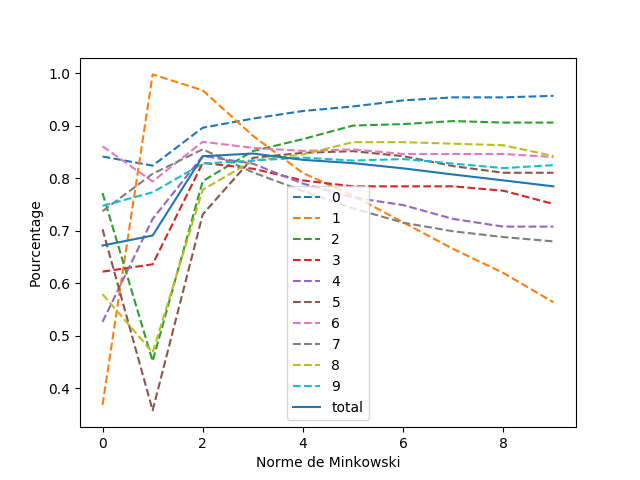
\includegraphics[width=\linewidth]{Graphs/normsminky.png}
  	\caption{Performance de l'algorithme pour chaque chiffre et en moyenne en fonction de la norme de Minkowsky (la valeur 0 en abscisse représente la norme infinie).}
\end{figure}

On remarque qu'en moyenne les normes 2 et 3 sont les plus performantes et aussi celles pour lesquelles les résultats obtenus pour les différents chiffres sont les plus proches. \\
La distance associée à la norme infinie ne prenant en compte que l'écart maximal composante par composante entre deux vecteurs, appliquée à la comparaison d'image elle est inefficace car l'écart maximal n'est pas représentatif de l'ensemble de l'image. De plus, quand k augmente, le comportement de la norme k de Minkowski tend vers celui de la norme infinie, ce qui se vérifie dans les résultats obtenus.\\ 
Pour la norme 1, on observe de mauvais résultats moyens avec beaucoup de disparités entre les différents chiffres(Figure 3.1). On a donc cherché à savoir lorsqu'un chiffre est mal reconnu avec quel chiffre il a été le plus confondu (Table 3.2).\\
On remarque pour la norme 1 que les 1 sont toujours correctement identifiés, mais que les autres chiffres sont souvent confondus avec des 1.

\begin{center}
\captionof{table}{Représente pour les normes 1,2 et 3 et pour un chiffre i donné avec quel autre chiffre le chiffre i est le plus souvent confondu par l'algorithme}
\begin{tabular}{ |c||c|c|c|c|c|c|c|c|c|c|c| } 
\hline
 Norme & 0 & 1 & 2 & 3 & 4 & 5 & 6 & 7 & 8 & 9 \\ 
  \hline
  \hline
  1 & 1 & 1 & 1 & 1 & 1 & 1 & 1 & 1 & 1 & 1 \\
 \hline
  2 & 5 & 8 & 1 & 8 & 9 & 3 & 1 & 9 & 1 & 4 \\
 \hline
  3 & 5 & 8 & 8 & 8 & 9 & 3 & 2 & 9 & 3 & 4 \\
 \hline
\end{tabular}
\end{center}


\chapter{Deuxième méthode : utilisation de la décomposition en valeurs singulière}
\subsection{Théorie}
Étant donné les résultats décevants de notre première méthode, il est nécessaire d'utiliser une autre technique qui prenne en compte les variations entre les différentes images représentant un même chiffre, cette technique repose sur un outil mathématique très puissant: la décomposition en valeurs singulières (SVD par ses initiales en anglais \textit{Singular Value Decomposition}).\\
Il s'agit ici dans un premier temps, de créer pour chaque chiffre (on parlera ici uniquement des trois pour alléger l'écriture) une matrice A de 784 lignes, comportant autant de colonnes que le nombre de 3 dont on dispose dans notre base d’entraînement. Chaque colonne de cette matrice représente une image de 3. On dispose alors d'un sous espace vectoriel de $\textbf{R}^{784}$ , engendré par les colonnes de A (on appellera cet espace vectoriel "l'espace des trois"), qui est nécessairement de faible dimension, sinon les espaces propres à chaque chiffre s'intersecteraient. Or le théorème de décomposition en valeurs singulières, nous permet de décomposer cette matrice ainsi: $$A = \sum_{i=1}^{784}{\sigma_{i}u_{i}v_{i}^{T}}$$\\
Les $u_{i}$ sont alors une base orthonormée de l'espace des trois. De plus lors d'une SVD, la base est ordonnée de manières à ce que les $\sigma_{i}$ forment une suite décroissante, qui dans notre cas finit par s'annuler. Les premiers vecteurs u de la SVD sont alors représentatifs de l'espace vectoriel des 3, étant donné que toutes les matrices de la somme sont de norme 1. On peut donc construire un espace des trois réduit ayant pour base (orthonormée) les premiers vecteurs u de la SVD. Ce sous-espace est de faible dimension par rapport à l'espace de dimension 784 dans le quel il vit et il est donc très peu probable qu'il intersecte le sous-espace relatif à un autre chiffre, ce qui garantit que les différents espaces réduits seront bien distincts dans le calcul à venir.\\
Maintenant qu'on dispose d'un espace vectoriel des 3 réduit (doté d'une base orthonormé), on peut facilement calculer la distance, pour la norme deux, du chiffre non identifié (c'est à dire un vecteur de  $\textbf{R}^{784}$) à cet espace (cela revient à un calcul des moindres carrés). Si on effectue ce calcul pour l'espace correspondant à chaque chiffre on peut alors labelliser l'image, en constatant de quel espace vectoriel elle est le plus proche.

\subsection{Pratique}

Pour cette méthode, nous avons effectué une classification (clustering) plus fine des résultats : si lors de l'analyse d'une image, on ne peut l'identifier de façon décisive à un chiffre, celle-ci est rejetée, ce qui permet d'améliorer le taux d'identification correct parmi les images non rejetées. \\
Plus précisément, une image $z$ sera rejetée si le minimum $m1$ de l'ensemble des $ \norm{(I-U_{k}U_{k}^{T})z}_{2}$ (les moindres carrés pour chaque chiffre) n'est pas "significativement" plus petit que le deuxième plus petit élément de cet ensemble $m2$ (deux bases de chiffres pourraient alors correspondre à l'image). Pour définir ce "significativement" nous avons introduit un seuil compris entre $0.5$ et $1$ : une image sera rejetée si après le calcul de ses moindres carrés $m1>seuil*m2$. Plus le seuil est bas plus l'on est exigeant : avec un seuil de $1$ aucune image n'est rejetée et avec un seuil de $0.5$ l'évaluation d'une image est jugée concluante seulement si $m1\leq 0.5m2$.


\begin{figure}[H]
\begin{center}
  	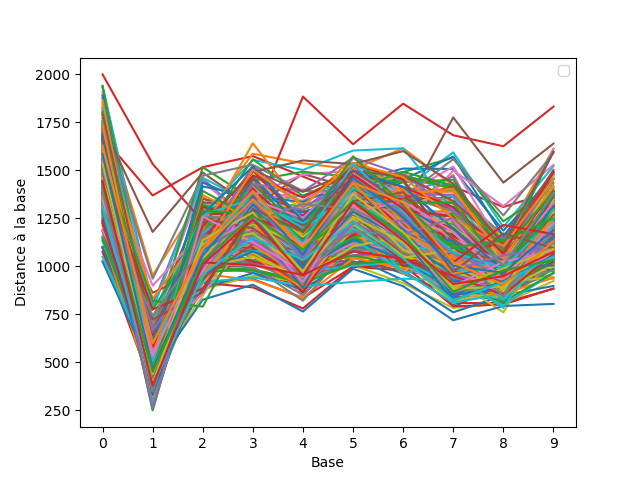
\includegraphics[width=0.7\linewidth]{Graphs/Distance_bases_20_1.png}
  	\caption{Distance pour chaque image de 1 aux espaces vectoriels (de dimension 20) représentant les différents chiffres. On remarque que les images sont bien plus proches de l'espace des uns que des autres espaces et il y a donc très peu d'erreur.}
  	\end{center}
\end{figure}

\begin{figure}[H]
\begin{center}

  	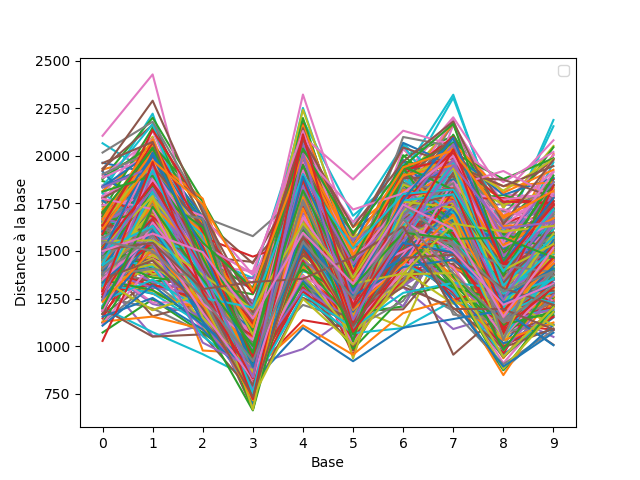
\includegraphics[width=0.7\linewidth]{Graphs/Distance_bases_20_3.png}
  	\caption{Distance pour chaque image de 3 aux espaces vectoriels (de dimension 20) représentant les différents chiffres. On peut remarquer des pics secondaires pour les espaces des 5 et des 8 ce qui signifie que les 3 sont plus difficiles à identifier clairement que les 1 et seront généralement pris pour des 5 et des 8 par l'algorithme lorsqu'il se trompera.}
\end{center}
\end{figure}


\subsection{Paramètres}
Nous avons cherché à optimiser cette deuxième méthode en jouant sur deux paramètres : le nombre de vecteurs de base de $U$ choisis $k$ et le seuil.\\

Le premier jeu de test a été effectué pour des valeurs du seuil entre 0.9 et 1 (des valeurs inférieures du seuil donnant un taux de rejet trop élevées env. 20\%) et une valeur de k (nombre de vecteurs de base) entre 1 et 7 (Figure 4.1).\\

\begin{figure}[H]
  	\includegraphics[width=\linewidth]{"Graphs/3D TP vs Rejected".png}
  	\caption{A gauche, pourcentage d'images correctement identifiées et a droite, pourcentage d'images rejetées en fonction de nombre de vecteurs de base et du seuil de distance minimale}
\end{figure}

On remarque que quelque soit la base, l'efficacité de l'algorithme évolue approximativement de la même manière en fonction de la valeur du seuil. \\ 
On peut donc par la suite se permettre d'étudier indépendamment l'influence du seuil et celle du nombre de bases.\\

\subsubsection{Seuil}

\begin{figure}[H]
  	\includegraphics[width=\linewidth]{"Graphs/TP vs Rejected".png}
  	\caption{Pourcentage de vrai positifs et de rejetés en fonction du niveau du seuil.}
\end{figure}

On remarque dans la figure 4.2 le pourcentage de vrais positifs et le pourcentages de rejetés sont proportionnelles et linéairement décroissantes en fonction du seuil. On n'a donc pas de choix optimal objectif pour le seuil, on choisira donc le seuil en fonction de la tolérance à l'erreur et le taux de rejet acceptable. 

\subsubsection{Nombre de vecteurs de base}
On remarque que l'efficacité de l'algorithme est croissante en fonction du nombre k de vecteurs de bases pour ceux observés. Cependant après notre analyse théorique, on peut dire que si k devient trop grand, les espaces vectoriels qu'on associe à chaque chiffre (étant de dimension k) ont de fortes chances de s'intersecter (Figure 4.3). Il est donc intéressant de chercher la valeur de k optimale pour notre algorithme.

\begin{figure}[H]
  	\includegraphics[width=\linewidth]{"Graphs/test30bases".png}
  	\caption{Performance pour chaque chiffre et en moyenne en fonction du nombre de vecteurs de base. A gauche lorsque le nombre de vecteurs de base est encore faible l'algorithme devient plus performant en augmentant ce paramètre. A droite on assiste à l'effondremment du modèle lorsque le nombre de vecteurs de base est trop élevé et que les espaces relatifs à chacun des nombres s'intersectent.}
\end{figure}

En faisant varier k entre 1 et 30, on remarque que l'efficacité de l'algorithme se stabilise à partir de k=20.De plus le nombre de vecteurs de base $k$ choisi n'influe pas significativement sur la complexité des calculs : en effet seul le calcul de $I-U_{k}U_{k}^{T}$ dépend de $k$ et il est effectué une seule fois pour chaque chiffre. On fixe donc par la suite k=20.

\chapter{Distance tangente}
\subsection{Théorie}
On souhaite désormais affranchir notre algorithme des erreurs liées aux petites variations usuelles que nos chiffres peuvent connaître lorsque qu'un humain les écrits. En effet il est courant dans une base de données réelle que les chiffres soient légèrement décalés, dilatés ou encore épaissis. Afin d'expliciter la méthode plus simplement, on va d'abord s’intéresser uniquement à rendre notre algorithme insensible à la translation en X. \\
Si on considère une image I comme un point dans $\textbf{R}^{784}$, l'ensemble des I translatés est une courbe continue dans $\textbf{R}^{784}$. On peut décrire l'ensemble des points de cette courbe, comme l'image de $\textbf{R}$ par la fonction f(x) = s(I,x), où s(I,$\alpha$) est l'élément de  $\textbf{R}^{784}$ correspondant à I décalé de $\alpha$ sur l'axe des X. P étant un autre élément de $\textbf{R}^{784}$, on cherche alors à établir la distance minimale entre un translaté de I et de P. Idéalement on aimerai donc définir la distance suivante, : $$d(I,P)= min_{\alpha,\beta \in \textbf{R}} ||s(I,\alpha)-s(P,\beta)||$$. 
Cependant il serait inutile d'essayer d'implémenter cette distance, puisque son calcul est très complexe et qu'on ne s’intéresse ici qu'à de petites translations. On va donc utiliser des approximations à l'ordre 1 des courbes des translatés, valables pour des petites valeurs de $\alpha$ et $\beta$. On effectue un développement de Taylor et on obtient:$$s(I,\alpha)\approx s(I,0) + \frac{ds}{d\alpha}(I,0)*\alpha=I + \frac{ds}{d\alpha}(I,0)*\alpha$$.
Ainsi on peut définir une nouvelle distance plus simple, à peu près équivalente au voisinage de 0: $$d_{2}(I,P)= min_{\alpha,\beta \in \textbf{R}} ||I+\frac{ds}{d\alpha}(I,0)*\alpha-P-\frac{ds}{d\beta}(P,0)*\beta)||$$
Or $\frac{ds}{d\alpha}(I,0)$ est indépendant de $\alpha$, on peut donc le noter $T_{I}$ et ainsi réécrire notre distance ainsi: $$d_{2}(I,P)= min_{\alpha,\beta \in \textbf{R}} ||(I-P)-\begin{pmatrix}-T_{I} & T_{P}\end{pmatrix} \begin{pmatrix}\alpha \\ \beta\end{pmatrix} ||$$ 
A condition que la norme utilisée soit la norme euclidienne, le calcul de cette distance est un problème des moindres carrés. On le résout grâce au théorème suivant : soit $A$ une matrice de rang plein de décomposition en valeurs singulières $A = U\Sigma V^T$, le problème des moindres carrés $min_x\norm{Ax-b}_2$ a pour unique solution $$x = V\Sigma^{-1}U_1^Tb$$ Ici $A = \begin{pmatrix}-T_{I} & T_{P}\end{pmatrix}$ et $b = (I-P)$.\\
 \\
Généralisons maintenant cette méthode au cas où l'image I peut avoir subit n transformations continues distinctes. L'espace affine des éléments correspondant aux I transformés, noté $C_{I}$ est alors de dimension n, car il est engendré par n courbes de dimension 1 (on peut à partir de I se déplacer dans $\textbf{R}^{784}$ suivant n courbes pour obtenir un I transformé, on voit bien qu'on peut décrire cet espace avec n paramètres). Soit P un autre élément de $\textbf{R}^{784}$ on souhaiterait comme précédemment pouvoir calculer la distance minimale entre $C_{I}$ et $C_{P}$ mais c'est impossible. On utilise donc à nouveau l'hypothèse que les transformations sont de petite ampleur, et on va approximer $C_{I}$ et $C_{P}$ par leur plans tangents en 0. Soit $\alpha$ dans $\textbf{R}^{n}$,on définit s la fonction tel que s(I,$\alpha$) soit l'élément de $\textbf{R}^{784}$ correspondant à I ayant subit pour tout i inférieur à n, la i-ème transformation avec un coefficient $\alpha_{i}$. $C_{I}$ est alors l'image par f(x)=s(I,x) de $\textbf{R}^{n}$, un développement de Taylor à l'ordre 1 permet alors d'expliciter le plan tangent à $C_{I}$ en 0. Au voisinnage de 0 on a:$$f(x) = s(I,x) \approx I + \sum_{i=1}^{n}\frac{ds}{d\alpha_{i}}(I,0)\alpha_{i}$$ On définit alors la distance tangente entre I et P comme la distance euclidienne minimale entre un point du plan tangent de I et un point du plan tangent de P:$$d_{tangente}(I,P)=min_{\alpha,\beta \in \textbf{R}^{n}}||I-P+\begin{pmatrix}-T_{I} & T_{P}\end{pmatrix} \begin{pmatrix}\alpha \\ \beta\end{pmatrix}$$ $$\textrm{où $T_{I}$ est la matrice des dérivées partielles de s(I,$\alpha$) selon $\alpha$.}$$\\
Il ne reste désormais plus qu'à réaplliquer notre premier algorithme en utilisant cette distance tangente, afin d'obtenr un code insensible aux modifications humaines usuelles.

\subsection{Pratique}

Pour implémenter l'algorithme on considérera les transformations suivantes : la translation (en x et en y), la rotation, l'agrandissement et le rétrécissement, l'étirement (horizontal, vertical et diagonal), et l'épaississement. On implémente chaque transformation et sa dérivée.\\
Par la suite on considérera les images comme des fonctions de deux variables $p(x,y)$ et on notera les dérivées partielles par rapport à x et y respectivement $p_x = \frac{dp}{dx}$ et $p_y = \frac{dp}{dy}$. Les images étant discrètes on calcule les dérivées par différences finies. 

\subsubsection{Translation}
La translation en $x$ de $\alpha_x$ pixels est donnée par la fonction $$s(p,\alpha_x)(x,y) = p(x+\alpha_x,y)$$ 
En utilisant le développement de Taylor à l'ordre 1, on obtient :
$$\frac{d}{d\alpha_x}(s(p,\alpha_x)(x,y))|_{\alpha_x=0} = \frac{d}{d\alpha_x}p(x+\alpha_x,y)|_{\alpha_x=0}=p_x(x,y)$$ 
De façon analogue on obtient la translation en y et sa dérivée.

\subsubsection{Rotation}
La rotation d'angle $\alpha_r$ est donnée par la fonction $$s(p,\alpha_r)(x,y) = p(x\cos\alpha_r+y\sin\alpha_r,-x\sin\alpha_r+y\cos\alpha_r)$$ 
Et sa dérivée par :
$$\frac{d}{d\alpha_r}(s(p,\alpha_r)(x,y))= (-x\sin\alpha_r+y\cos\alpha_r)p_x - (x\cos\alpha_r+y\sin\alpha_r)p_y$$
d'où
$$\frac{d}{d\alpha_r}(s(p,\alpha_r)(x,y))|_{\alpha_r=0}=yp_x-xp_y$$ 
où les dérivée sont évaluées en $(x,y)$

\subsubsection{Agrandissement et rétrécissement}
Les fonctions de changement d'échelle sont donnée par : $$s(p,\alpha_s)(x,y) = p((1+\alpha_s)x,(1+\alpha_s)y)$$  
Et sa dérivée par :

$$\frac{d}{d\alpha_s}s(p,\alpha_s)(x,y)|_{\alpha_s=0}=xp_x+yp_y$$ 

\subsubsection{Étirement}
L'étirement horizontal ou vertical est donné par : $$s(p,\alpha_p)(x,y) = p((1+\alpha_p)x,(1-\alpha_p)y)$$  
Et sa dérivée par :

$$\frac{d}{d\alpha_p}s(p,\alpha_p)(x,y)|_{\alpha_p=0}=xp_x-yp_y$$ 

L'étirement diagonal est donné par : $$s(p,\alpha_p)(x,y) = p(x+\alpha_py,y+\alpha_px)$$  
Et sa dérivée par :

$$\frac{d}{d\alpha_p}s(p,\alpha_p)(x,y)|_{\alpha_p=0}=yp_x+xp_y$$ 

\subsubsection{Épaississement}
Pour l'épaississement on considérera seulement la dérivée \cite{Elden} : $$(p_x)^2+(p_y)^2$$

\subsubsection{Comparaison entre la distance euclidienne et la distance tangente}
Notre algorithme différe de celui des écarts à la moyenne uniquement par la distance utilisée. Il est donc intéressant de comparer la distance d'un 3 modifié à la moyenne de chaque chiffre en fonction de la distance choisie et de l'intensité de la modification. Dans le cas où la transformation est l'identité, les distances sont égales car le 3 utilisé est le 3 moyen.

\begin{figure}[H]
  	\includegraphics[width=\linewidth]{"Graphs/GraphesOct".png}
  	\caption{Distances des images moyennes à l'image moyenne des 3 translaté horizontalement en fonction de la valeur translation.}
\end{figure}

On remarque qu'avec la distance euclidienne, un décalage de 2 pixels vers la gauche de l'image suffit à avoir une mauvaise identification, alors que pour la distance tangente, on identifie correctement l'image même après des décalages allant jusqu'à 6 pixels.


\subsection{Algorithme}
On calcule pour chaque chiffre la moyenne des images du jeu d'entraînement (comme dans le premier algorithme) puis on calcule la matrice des dérivées de chaque transformation appliquée à chaque image moyenne. Pour tester une image, on calcule de même la matrice des dérivées pour celle-ci. On l'identifie ensuite au chiffre tel que la distance tangente à l'image moyenne associée soit minimale.



\subsection{Tests}
Pour vérifier l'efficacité de l'algorithme, nous avons implémenté les différentes transformations à l'aide des modules python de traitement d'image (scipy et openCV) et généré des jeux de tests où chaque image a subi un nombre de transformations aléatoirement choisies. On a ensuite comparé l'efficacité de cet algorithme avec les deux autres algorithmes.\\
Nous avons crée trois bases de test, avec différentes niveaux de "bruit": chaque image subit une, deux ou trois transformations choisies aléatoirement.

%Tableau test 3 algos
\begin{center}

\captionof{table}{Performance des trois algorithmes sur une base ayant subi une transformation}
\begin{tabular}{ |c||c|c|c|c|c|c|c|c|c|c|c| } 
\hline
 Algorithme & 0 & 1 & 2 & 3 & 4 & 5 & 6 & 7 & 8 & 9 & \textbf{Total} \\ 
  \hline
  \hline
  1 & 72.0 & 85.3 & 65.4 & 62.6 & 74.7 & 59.7 & 75.O & 73.9 & 57.1 & 61.4 & \textbf{69.0} \\
 \hline
  2 & 97.3 & 94.4 & 94.0 & 94.8 & 96.9 & 94.7 & 95.1 & 95.0 & 91.3 & 91.6 & \textbf{94.6} \\
  \hline
  3 & 84.8 & 92.5 & 73.2 & 78.4 & 86.4 & 75.9 & 86.0 & 83.7 & 66.7 & 72.9 & \textbf{80.3} \\
 \hline
\end{tabular}

\captionof{table}{Performance des trois algorithmes sur une base ayant subi deux transformations}
\begin{tabular}{ |c||c|c|c|c|c|c|c|c|c|c|c| } 
\hline
 Algorithme & 0 & 1 & 2 & 3 & 4 & 5 & 6 & 7 & 8 & 9 & \textbf{Total} \\ 
  \hline
  \hline
  1 & 58.9 & 72.8 & 57.4 & 51.8 & 67.5 & 53.1 & 61.2 & 64.7 & 46.0 & 46.3 & \textbf{58.2} \\
 \hline
  2 & 94.0 & 87.5 & 91.2 & 91.2 & 93.3 & 93.6 & 92.3 & 91.9 & 88.8 & 85.3 & \textbf{90.9} \\
  \hline
  3 & 73.4 & 82.4 & 67.5 & 69.1 & 79.9 & 71.7 & 73.9 & 75.2 & 57.4 & 62.1 & \textbf{71.4} \\
 \hline
\end{tabular}

\captionof{table}{Performance des trois algorithmes sur une base ayant subi trois transformations}
\begin{tabular}{ |c||c|c|c|c|c|c|c|c|c|c|c| } 
\hline
 Algorithme & 0 & 1 & 2 & 3 & 4 & 5 & 6 & 7 & 8 & 9 & \textbf{Total} \\ 
  \hline
  \hline
 1 & 47.0 & 66.9 & 50.7 & 41.3 & 61.2 & 47.6 & 50.7 & 54.2 & 37.4 & 35.3 & \textbf{49.5} \\
 \hline
 2 & 92.9 & 82.4 & 90.3 & 83.8 & 90.6 & 89.5 & 89.7 & 88.4 & 85.4 & 77.3 & \textbf{87.1} \\
  \hline
 1 & 62.8 & 76.8 & 61.7 & 58.9 & 73.6 & 65.0 & 66.2 & 66.2 & 48.2 & 52.8 & \textbf{63.4} \\
 \hline
\end{tabular}
\end{center}

On remarque que la distance tangente permet d’améliorer substantiellement la résistance au bruit de l'algorithme des écarts a la moyenne. Cependant la méthode de décomposition en valeurs singuliers offre des meilleurs résultats, même sur un base bruitée.

\chapter{Test globaux}

Pour tester la performance des algorithmes implémentées on a effectué une série de tests sur l'ensemble de la base de donnée: on a réservé 20\% des images de la base de données comme ensemble de test, puis nous avons sélectionné aléatoirement la moitié des images restantes comme ensemble d’entraînement.\\
Pour évaluer la complexité en temps de calcul, on a exécuté chaque algorithme sur un ensemble de 1000 images avec les résultats suivants: l'algorithme des écarts à la moyenne prend 0.1 secondes, celui de la décomposition en valeurs singulières 37.7 secondes et celui de la distance tangente 1137.9 secondes (environ 20 minutes).

\subsection{Écarts a la moyenne}
Pour le premier algorithme nous avons testé 50 fois, obtenant en moyenne des performances (taux d'identification correct) de 83\% pour la norme 2 et 84\% pour la norme 3 (Table 5.1) avec des résultats variées en fonction des chiffres analysés.

\begin{center}
\captionof{table}{Performance Algorithme 1, pour les normes 2 et 3}
\begin{tabular}{ |c||c|c|c|c|c|c|c|c|c|c|c| } 
\hline
 Norme & 0 & 1 & 2 & 3 & 4 & 5 & 6 & 7 & 8 & 9 & \textbf{Total} \\ 
  \hline
  \hline
  2 & 88.2 & 96.4 & 77.2 & 81.7 & 83.9 & 70.3 & 87.9 & 85.7 & 75.8 & 79.5 & \textbf{83} \\
 \hline
  3 & 90.2 & 88.6 & 84.6 & 80.7 & 82.5 & 80.7 & 88.0 & 82.1 & 82.2 & 79.9 & \textbf{84} \\
 \hline
\end{tabular}
\end{center}

\subsection{Décomposition en valeurs singuliers}
L'algorithme de décomposition en valeurs singuliers étant significativement plus coûteux quant au temps de calcul, on a effectuée 30 tests, obtenant une performance moyenne de 96\% avec un minimum de 94\% (Table 5.2). Les performances sont significativement plus consistantes pour toutes les chiffres par rapport à l'algorithme d'écarts a la moyenne.

\begin{center}
\captionof{table}{Performance Algorithme 2 avec 20 vecteurs base}
\begin{tabular}{ |c||c|c|c|c|c|c|c|c|c|c|c| } 
\hline
 Chiffre & 0 & 1 & 2 & 3 & 4 & 5 & 6 & 7 & 8 & 9 & \textbf{Total} \\ 
  \hline
  \hline
  Performance & 98.9 & 99.2 & 94.6 & 94.8 & 97.1 & 94.3 & 97.9 & 94.8 & 93.9 & 94.4 & \textbf{96.0} \\ 
\hline
\end{tabular}
\end{center}

En ajoutant un seuil de ressemblance minimale, on est capable de mettre de coté les chiffres les plus difficiles à identifier (Tables 5.3 et 5.4). si on accepte un taux de rejet d'environ 5\% on peut atteindre un pourcentage d'identification correcte d'environ 98\%.

\begin{center}
\captionof{table}{Performance et taux de rejet de l'Algorithme 2 avec 20 vecteurs base et un seuil de 0.99, pour les chiffres de 0 à 9 et en moyenne.}
\begin{tabular}{ |c||c|c|c|c|c|c|c|c|c|c|c| } 
 \hline
   & 0 & 1 & 2 & 3 & 4 & 5 & 6 & 7 & 8 & 9 & \textbf{Total} \\ 
  \hline
  \hline
 Performance & 99.0 & 99.3 & 95.1 & 95.5 & 97.4 & 95.2 & 98.1 & 95.5 & 94.8 & 95 &  \textbf{96.6} \\
  \hline
 Rejetées & 0.2 & 0.1 & 1.1 & 1.6 & 0.7 & 1.9 & 0.4 & 1.4 & 1.7 & 1.3 & \textbf{1.0} \\
 \hline
\end{tabular}
\end{center}


\begin{center}
\captionof{table}{Performance et taux de rejet de l'Algorithme 2 avec 20 vecteurs base et un seuil de 0.95, pour les chiffres de 0 à 9 et en moyenne.}
\begin{tabular}{ |c||c|c|c|c|c|c|c|c|c|c|c| } 
 \hline
   & 0 & 1 & 2 & 3 & 4 & 5 & 6 & 7 & 8 & 9 & \textbf{Total} \\ 
  \hline
  \hline
 Performance & 99.5 & 99.6 & 96.7 & 97.7 & 98.7 & 97.9 & 98.9 & 97.5 & 97.5 & 97.4 &  \textbf{98.2} \\
  \hline
 Rejetées & 1.2 & 0.6 & 5.1 & 7.6 & 4.1 & 9.9 & 2.5 & 6.7 & 9.2 & 6.5 & \textbf{5.3} \\
 \hline
\end{tabular}
\end{center}

\subsection{Distance tangente}
L’algorithme de distance tangente étant très coûteux en temps de calcul (environ 40 fois plus lent que le deuxième en 10000 fois plus lent que le premier),on a effectuée 10 test sur la base de données obtenant une performance moyenne de 89.6\% (Table 6.5).\\
Cette performance si bien est plus élevée que celle du premier algorithme, reste très inférieure a celle de l'algorithme SVD. 
%Ajouter une phrase disant que l'utilisation dans la vraie vie est impraticable (je n'ai pas d'imagination en ce moment ci)

\begin{center}
\captionof{table}{Performance algorithme distance tangente pour les chiffres de 0 à 9 et moyenne.}
\begin{tabular}{ |c||c|c|c|c|c|c|c|c|c|c|c| } 
 \hline
   & 0 & 1 & 2 & 3 & 4 & 5 & 6 & 7 & 8 & 9 & \textbf{Total} \\ 
  \hline
  \hline
 Performance & 94.9 & 99.6 & 79.2 & 92.5 & 90.3 & 83.6 & 94.5 & 90.9 & 80.7 & 88.0 &  \textbf{89.6} \\

 \hline
\end{tabular}
\end{center}


\chapter{Conclusion}
En comparant les résultats obtenus avec ceux de l'ouvrage de référence (Elden, 2007) on remarque que l'on a de meilleurs performances avec les deux premiers algorithmes. On peut expliquer cela par le fait la base que nous avons utilisée est environ 7 fois plus grande et que les images traitées ont une résolution plus élevée ($28\times 28$ par rapport à $16\times 16$ pixels dans l'ouvrage de référence).\\
Pour l'algorithme des distances tangentes, Elden compare les images à tester à chaque image du jeu d'entraînement. Bien que cela donne de bon résultats, pour l'ensemble de données utilisé et les ressources informatiques à notre disposition, cette implémentation est irréalisable. Nous avons donc implémenté la distance tangente comme une amélioration de l'algorithme des écarts à la moyenne. 

\bibliographystyle{ieeetr}
\bibliography{Bibliographie}
%\nocite{*} 
\end{document}
